% !TeX encoding = UTF-8
% !TeX spellcheck = pl_PL
\documentclass{article}
\newcommand\tab[1][1cm]{\hspace*{#1}}
\usepackage[]{polski}
\usepackage[utf8]{inputenc}
\usepackage{graphicx}
\usepackage{float}
\usepackage{amsmath}
\usepackage{geometry}
 
\usepackage{listings}
\usepackage{color, colortbl}
\usepackage{hyperref}

\usepackage{multirow}
\usepackage{pdfpages}

\usepackage[
separate-uncertainty = true,
multi-part-units = repeat
]{siunitx}

\definecolor{codegreen}{rgb}{0,0.6,0}
\definecolor{codegray}{rgb}{0.5,0.5,0.5}
\definecolor{codepurple}{rgb}{0.58,0,0.82}
\definecolor{backcolour}{rgb}{0.95,0.95,0.92}

\lstdefinestyle{mystyle}{
	backgroundcolor=\color{backcolour},   
	commentstyle=\color{black},
	keywordstyle=\color{blue},
	numberstyle=\tiny\color{codegray},
	stringstyle=\color{codepurple},
	basicstyle=\footnotesize,
	breakatwhitespace=false,         
	breaklines=true,                 
	captionpos=b,                    
	keepspaces=true,                 
	%numbers=left,                    
	%numbersep=5pt,                  
	showspaces=false,                
	showstringspaces=false,
	showtabs=false,                  
	tabsize=2
}

\lstset{style=mystyle}
\date{}

\author{Kamila Lis}

\title{Rozpoznawanie loga warszawskiego metra\\
	{\large Dokumentacja projektu z przedmiotu Przetwarzanie Cyfrowe Obrazów (POBR)}}

\begin{document}
	\maketitle
%	\begin{figure}[h]
%		\centering
%		\includegraphics[width=1\textwidth]{images/wybor_cech.png}
%		\caption{Wykres wartości cech 2 i 4.}
%		\label{24}	
%	\end{figure}

% wstępnego przetworzenia, segmentacji, wyznaczania cech oraz identyfikacji obrazów cyfrowych
\section{Treść zadania}
Dla indywidualnie wybranej klasy obrazów dobrać, zaimplementować i przetestować odpowiednie procedury wstępnego przetworzenia, segmentacji, wyznaczania cech oraz identyfikacji obrazów cyfrowych. Powstały w wyniku projektu program powinien poprawnie rozpoznawać wybrane obiekty dla reprezentatywnego zestawu obrazów wejściowych. W trakcie projektu należy przetestować wybrane algorytmy i ocenić ich praktyczną przydatność.

\section{Działanie programu}
Program wykrywa na zdjęciach logo warszawskiego metra. Znalezione loga zostają obramowane. Sekwencje przetwarzania jest następująca:
\begin{enumerate}
	\item \textbf{Progowanie w przestrzeni HSV} \\
	W pierwszej kolejności, aby umożliwić wyodrębnić żółte i czerwone fragmenty niezależnie od oświetlenia danego obrazu, obraz przekształcany jest z przestrzeni RGB do HSV. Na podstawie podanego zakresu barw i nasyceń tworzone są maski dla obu kolorów (jeden kanał w zakresie 0-255, 0 - tło, 255 - poszukiwany kolor). Wartości progowe barwy (hue) i nasycenia (saturation) zostały wyznaczone na podstawie zdjęć testowych.
	\begin{figure}[h]
		\centering
		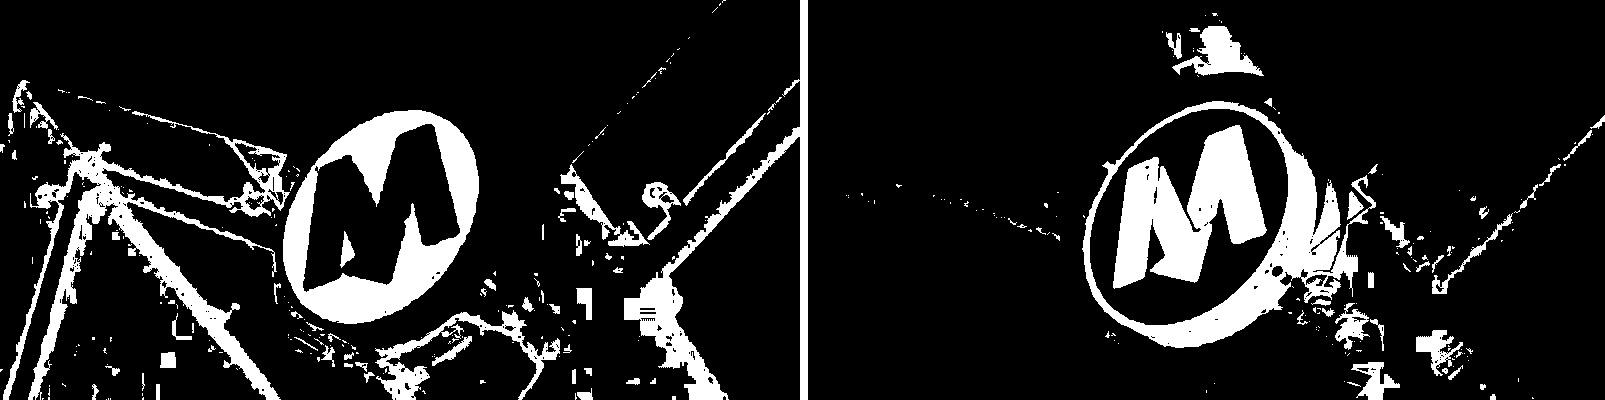
\includegraphics[width=1\textwidth]{masks.jpg}	
	\end{figure}
	\item \textbf{Redukcja szumów (filtr medianowy)} \\
	W celu redukcji pojedynczych białych pikseli maski (szumów) wykonywana jest filtracja medianowa z rozmiarem jądra równym 3. 
	\begin{figure}[h]
		\centering
		
\includegraphics[width=0.5\textwidth]{rankFilter.jpg}	
	\end{figure}
	\item \textbf{Segmentacja (etykietowanie obiektów)}\\
	Ponieważ poza poszukiwanym logiem inne obiekty na zdjęciu mogą spełniać warunek koloru, w kolejnym kroku wartości zapisane w masce koloru żółtego grupowane są w obiekty. Wykonywane jest to za pomocą etykietowania: dla każdego piksela, który nie jest tłem i nie ma przypisanej etykiety nadawana jest nowa etykieta. Następnie, rekurencyjnie, przypisywana jest ona wszystkim jego sąsiadom.
	\begin{figure}[h]
		\centering
		
\includegraphics[width=0.5\textwidth]{metro.jpg}	
	\end{figure}
	\item \textbf{Wyznaczanie cech}\\
	 Segment maski żółtej jest zaliczany jako logo, jeśli: 
	\begin{itemize}
		\item spełnia wymagania co do zakresu niezmiennika M3 oraz kształtu Malinowskiej,
		\item w prostokącie opisującym segment stosunek sumy pikseli czerwonych i żółtych do pola elipsy, określonego na podstawie wyznaczonego prostokąta, jest jednostkowy ($\pm 0.4$), 
		\item liczba pikseli czerwonych (w wyznaczonym prostokącie) jest nie mniejsza niż $\frac{1}{4}$ liczby pikseli żółtych.
	\end{itemize} 
	\begin{figure}[H]
		\centering
		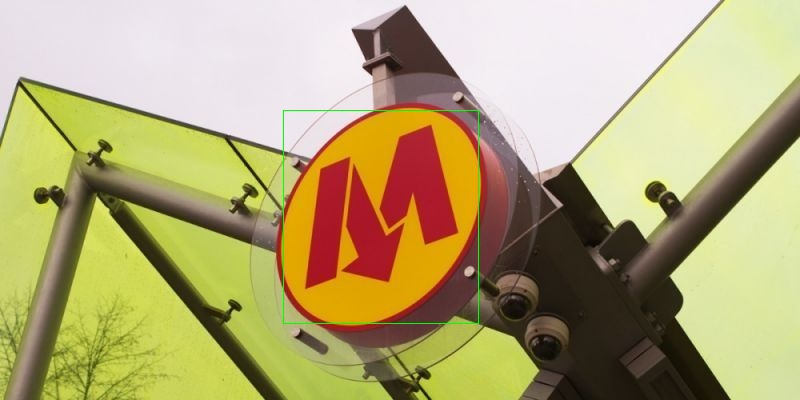
\includegraphics[width=0.5\textwidth]{image.jpg}	
	\end{figure}
\end{enumerate}

\section{Wnioski}
Zaimplementowany program wyznacza poprawnie wszystkie wystąpienia loga warszawskiego metra na zdjęciach przygotowanego zestawu testowego.

Istotnym ułatwieniem wyznaczania progów dla tworzenia masek wyodrębniających kolory było przeniesienie obrazu do przestrzeni HSV. Pozwoliło to na wykrywanie loga w różnych warunkach i teksturach. Możliwą perspektywą rozwoju programu jest zmiana algorytmu segmentacji na nierekurencyjną. 

	
\end{document}